\section{Task 1: Understanding HSRN researchers' needs and behaviors}

\begin{figure}[t]
    \centering
    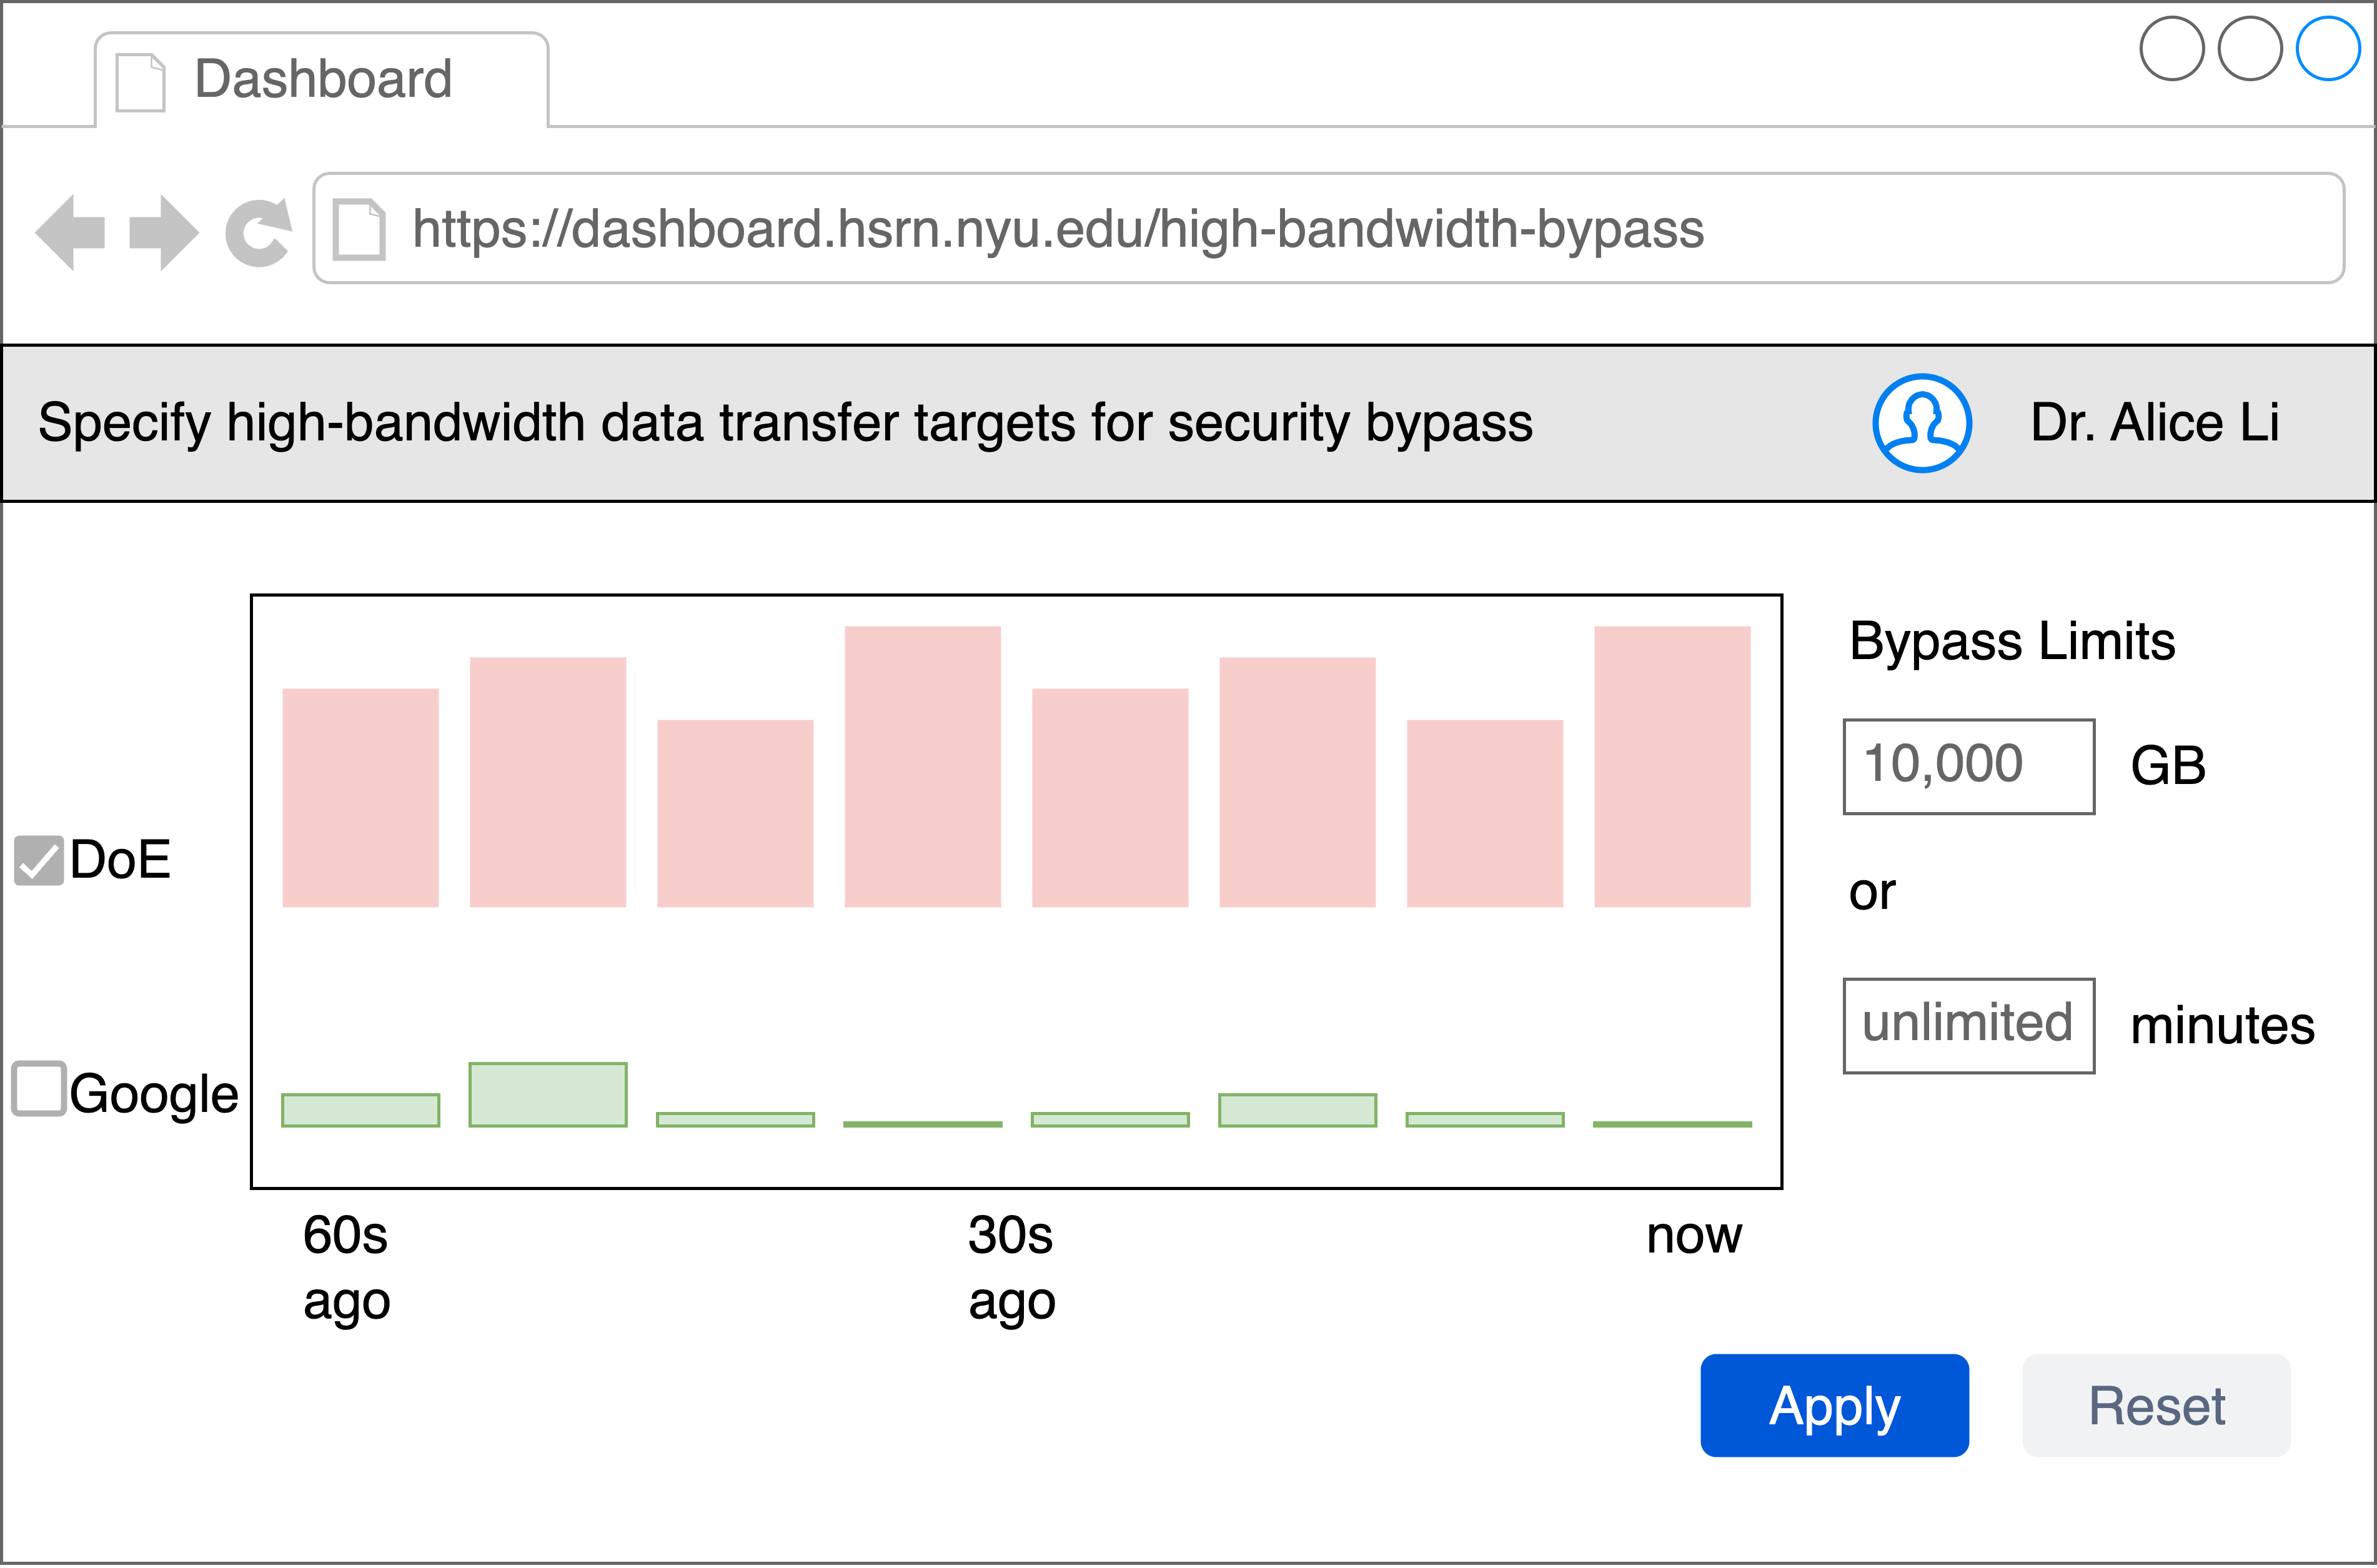
\includegraphics[width=0.7\linewidth]{figures/dashboard.png}
    \caption{A sample of the dashboard's user interface.}
    \label{fig:dashboard}
\end{figure}


Before we implement the system, we first need to understand the needs of researchers as reported by researchers, e.g., how they interact with the current HSRN, how they currently request security bypasses, what are their concerns, and what they would like to see as a solution. This human-centered understanding will help us design the user interface and user experience (UI/UX). We will provide the details in Task 1a.

In addition, we will also need to understand the researchers' behaviors as reported by the network traffic, e.g., their network activities and traffic patterns, by conducting passive network measurements. This analysis will facilitate the automatic annotation of the network traffic of users, e.g., which remote destinations the users are contacting and the estimated bandwidth and latency requirements. Such annotations will help researchers make informed decisions when requesting security bypasses in the UI/UX. We will provide the details in Task 1b.

\subsection{Task 1a: Understanding researchers' needs through user studies}

\paragraph{Understanding existing concerns}
Understanding concerns. Through surveys and semi-structured interviews, we plan to understand how they are currently using the HSRN and their experience with the network administrators.


So let's start with the first task first, basically, understanding the users behaviors and there needs so it breaks down into two sub parts under task number one, there's task number one A and task number one be task one A is understanding users needs. And task one B is understanding humans B users behaviors. So at a very high level, we want to understand human needs because we want to see basically what problems the users are running into in the current setup. Like right now we have a high speed Research Network.

But there are problems for example, you know, users might want you to might want to

ask for permission, make special requests, just so that they can, you know, put themselves into the DMZ so that they can enable high speed transfers or low latency transfers. But this is a very manual process, they have to submit requests to network administrator's open particular ports enable certain flows and applications are certain periods of time this is an error prone process is a manual process. We have seen instances where,

you know, a sysadmin would take weeks to enable this rule number one, and number two, sometimes this admin would forget to disable this rule leaving the user open to attacks. So you know, from the user's point of view, the researchers point of view, they're suffering from two problems in the current setup. One is that it's a long process manual process.

It is a bottleneck in their research. And two, they are exposed to unnecessary security risks. So these are the two problems you wanted to talk, we want to talk to researchers understand what other needs they have, what other pain points they have, during this process, and we need to ask them, basically,

if you have a new system, how would you design this? So achieve these goals? We wanted to do two things. One, is we want to conduct surveys and interviews and focus groups just to talk to them and understand, you know, what is the current workflow? For example? Are they faculty that do ar VR research that need a low latency network? Are they faculty in, for example, computational physics, I'm sorry, computational chemistry or physics that need to transfer large amounts of data that require high bandwidth in each of these cases? What are their current experiences? Like with the high speed network? Do the experience stillness in certain cases? Do they

need to talk to it to make special requests? What are in their special requests?

What specification are in a special request when it talks to it?

What are the interactions helpful with the interactions intuitive, presumably because IT departments was, you know, be highly technical, where these researchers are not trained in networking or security? Do they understand the interactions between it what they're doing? So these are some of the potential issues that are facing these researchers right now. And one, understand the current user experience through interviews, through focus groups, mostly semi structured interviews right now, and focus groups so that you know we didn't get all the problem understand the problems. So this is the first part. The second part is that we wanted to them to sit together in what we call the code design sessions, where they will be along with the researchers, they will come up with ways to design a solution that will suit their needs.
For example, in the ideal product, how would the interaction look like


In this code designs in these code design, co design sessions, what they will do is that they will sit down together with the researchers and come up with ways solutions, simple user interfaces, that will use their knees for example, specifying their workloads, you know, low latency workload versus high bandwidth workloads specifying visually, their requests IT departments, for example, opening particular ports, or how to specify destinations. For example, if you want to say, transfer files to do E, how would they represent the destination do E is if their IP addresses host names or what so we want to understand the ideal user interface for these researchers, especially given that many of them do not have a background in networking or security, what is the mental model about security in these cases? So that is pretty much task one a understanding the researchers need. So at the end of task one A, here is our expected outcome, we will come up with a set of qualitative analysis that shows the current experience and needs concerns of the researchers and will come up with rough sketches of the potential design for a dashboard. That would work for different needs of different researchers. That's task one a.




\paragraph{Understand traffic patterns}
Understand qualitatively what kind of network traffic they send. Elephant flows, or latency sensitive flows, presumably depending on what kind of experiment or research work they do.

\paragraph{Co-designing UI/UX}
We plan to co-design sessions in focus groups to make preliminary designs on what the dashboard looks like and the proposed user interactions. Make sure that our design is a part of their workflow. Depends on the traffic patterns. Some folks may have elephant flows. Some folks may have latency sensitive flows.

Understand how they want to express blessed destinations or network behaviors. end-users of open scientific infrastructure may consider security processes valuable only insofar as they do not slow or otherwise impede their research


\paragraph{Preliminary work}
Inspector dashboard, CHI paper dashboard

\paragraph{Expected outcome}
// From: Jeremy
-An open source tool to monitor,visualize and manage security and data transmission in academic high speed research neworks
-A dashboard front end that  provides remote management by researchers and network administrators. .

\paragraph{Lead investigator}
PI Huang will lead the study. He's done user studies before.






\subsection{Task 1b: Identifying traffic patterns through network measurement}

We need to help researchers make a decision. Bootstrap the allow list. Initial annotations.


In task one be our goal is to basically come up with default configurations for the allowed lists. At the end of the day, these researchers, we need to help them Bootstrap. Basically, when they first open the dashboard, the dashboard shows some default settings that already fit their needs. For example, if this is a physicist who regularly sends large amounts of data to say, the Department of Energy, the dashboard should come with pre configured settings for enabling transfers to Department of Energy. So we come up with these default values from two sources. One is from task one a where we find out you know, what the usual regular workflows from the visa researchers are based on their self reports. And based on, you know, this quality of qualitative data. That's the first source. The second source would be coming from network measurement data. We can look at these researchers network traffic. For example, for this physicist, we were able to identify things like this researcher does indeed send a large number of bytes to a server with a domain name that ends with do E and or the autonomous system number belongs to a D O E Network. This not only helps us This not only helps us confirm the user self report, but it also provides us with a set of quantitative metrics for just identifying the workflows, for example, the workflows will be in the form the the end of it is for a way for us to create annotations of their workflows for example, in this case, the work the annotation would be source coming from this researcher and destination going to particular IP address or the DNS would correspond to a doe domain. We will learn this data from several sources one from existing data collection mechanisms In a case of NYU, we have this thing called a net box that has analyzed data. Another way we propose is that we will stick this Zeke box into the network, which captures network traffic through a, a tap port, which mirrors the traffic, who is Zeke instance. And that would record basically what DNS traffic is captured. And also, what's the destination IP addresses. And various flow statistics like the total number of bytes, the duration of flows, and, you know, things like inter packet arrival times, which is important in characterizing low latency applications. So, basically, in summary, the second task, I'm sorry, task one B will help us generate a set of annotations for network traffic, that would quantitatively describe various workflows for these researchers, workflows, that are high bandwidth in nature, or workflows that are low latency in nature for different kinds of researchers. So that's task one, B.



\paragraph{Clustering flows} XXX

Clustering flows. Based on Task 1a, we know qualitatively what kinds of flows researchers tend to generate. Can we identify them? Can we cluster their network activities on the network and match against the qualitative study? For a data transfer, is it mostly elephant flows to a single destination vs mice flows?

\paragraph{Identifying destinations}
What about destinations? Let's say transfer to DoE — is it just one server, or multiple? External vs internal destinations?

\paragraph{Preliminary work} We spoke to some of the users about their work flows

// netbox already captures who is on which port and use case; flows to help us troubleshoot network speed.

no ipv6; too much work




On the dashboard users need to specify which of their network activities to add to an allow list. Not an easy process. Many flows on their computers, elephant and mice. Also multiple destinations, sometimes to CDNs. We help them make this decision.

Profiling users. Task 1a and 1b already give us user profiles.

Auto-identifying destinations. What destination are you talking to? Not straightforward. PI Huang has some preliminary work. NLP. Zeek logs

Auto-clustering traffic patterns. Identifying elephant flows and latency sensitive flows. Presenting this information through dashboard.  Zeek.

// Idea: identifying network flows

\paragraph{Preliminary work} Inspector work — identifying hosts, based on webXray. Flow clustering: PI Huang's HotSDN paper.

\paragraph{Expected outcome} A technique to automatically identify destinations and traffic patterns to help users make decisions more easily.

\paragraph{Lead investigator} PI Huang and Co-PI Pahle will work together on implementing. Co-PI Cappos will advise on XXX.



\paragraph{Expected outcome} A measurement analysis. Clusters per researcher and type of researcher.

\paragraph{Lead investigator} Co-PI Pahle will work with IT to conduct the study, as he's already a part of the NYU research IT infrastructure team. PI Huang to help with the anonymized data analysis. PI Huang is familiar with network measurement and big data analytics.
